\chapter{\IfLanguageName{dutch}{Framework- en parameterselectie}{Framework and parameter selection}}%
\label{ch:selectie}

\section{Parameters voor correcte uitvoering en foutdetectie bij basis krachtoefeningen}

\subsection{Inleiding}
Bij het ontwikkelen van een pose estimation model voor de analyse van krachttrainingsoefeningen is het essentieel om duidelijke parameters te definiëren die een correcte van een incorrecte uitvoering onderscheiden. 
Op basis van literatuuronderzoek worden hieronder de belangrijkste parameters voor squat, bench press en deadlift beschreven, samen met indicatoren voor incorrecte uitvoering die door het model gedetecteerd kunnen worden.

\subsection{Squat: parameters voor bewegingsanalyse}

\subsubsection{Correcte uitvoering}
De squat vereist een nauwkeurige coördinatie van verschillende lichaamssegmenten. 
Voor een correcte uitvoering dient de voetplaatsing op schouderbreedte of iets breder (circa 1,2-1,5 keer de schouderbreedte) te zijn, met de tenen recht naar voren of maximaal 7-10 graden naar buiten gedraaid \autocite{LorenzettiEtAl2018}. 
De gehele voet moet contact houden met de grond, waarbij vooral de hielen stevig moeten blijven staan \autocite{CzaprowskiEtAl2012}. 
De knieën dienen in lijn te blijven met de tenen, waarbij ze ongeveer 5-10 cm voorbij de tenen mogen komen in een hoek van zo'n 45 graden ten opzichte van de romp \autocite{LorenzettiEtAl2018}.

De diepte van de squat is minimaal 90 graden kniehoek (halve squat), of voor een volledige squat dienen de dijen parallel aan de grond te zijn (115-125 graden knieflexie) \autocite{ComfortEtAl2018}. 
De natuurlijke lumbale lordose (onderrug) moet behouden blijven, terwijl een thoracale kyfose (bolle bovenrug) vermeden dient te worden, met de romp onder een hoek van ongeveer 45 graden bij een volledige squat \autocite{CzaprowskiEtAl2012}.

De beweging begint met het naar achteren duwen van de heupen, gevolgd door een gecontroleerde afdaling (2-3 seconden) en een gecontroleerde opwaartse beweging (1-2 seconden) \autocite{CzaprowskiEtAl2012}.

\subsubsection{Incorrecte uitvoering en foutdetectie}
Bij de squat kan het pose estimation model de volgende veelvoorkomende fouten detecteren:

\begin{itemize}
    \item \textbf{Knieën naar binnen vallend (valgus)}: Wanneer de knieën tijdens de beweging naar binnen vallen ten opzichte van de voetlijn, verhoogt dit het risico op knieblessures \autocite{BengtssonEtAl2018}. 
    
    \item \textbf{Hielen die van de grond komen}: Het loskomen van de hielen duidt op een instabiele basis en verschuift het gewicht ongewenst naar de voorvoet \autocite{CzaprowskiEtAl2012}. 
    
    \item \textbf{Overmatige voorwaartse leun}: Een te grote voorwaartse kanteling van de romp verhoogt de schuifkrachten op de onderrug \autocite{BengtssonEtAl2018}. 
    
    \item \textbf{Bolle bovenrug (thoracale kyfose)}: Een verlies van de natuurlijke rugkromming verhoogt de druk op de tussenwervelschijven \autocite{CzaprowskiEtAl2012}. 
    
    \item \textbf{Ongecontroleerde beweging of stuiteren}: Een te snelle afdaling of stuiterende beweging onderaan de squat verhoogt de schuifkrachten op de knie \autocite{BengtssonEtAl2018}. 
    
    \item \textbf{Onvoldoende diepte}: Het niet bereiken van minimaal een 90-graden kniehoek vermindert de effectiviteit van de oefening \autocite{ComfortEtAl2018}. 
\end{itemize}

\subsection{Bench Press: parameters voor bewegingsanalyse}

\subsubsection{Correcte uitvoering}
Voor een correcte bench press is een stabiele lichaamspositie met vijf contactpunten essentieel: hoofd, schouderbladen, bovenrug en billen op de bank, met beide voeten stevig op de grond \autocite{KrolEtAl2010}. 
De handpositie vergt een bovenhandse greep waarbij de handen op ongeveer 1,5 keer de schouderbreedte staan, met de polsen stijf en recht boven de ellebogen \autocite{NoteboomEtAl2024}.

Bij de bewegingsuitvoering dienen de bovenarmen in een hoek van ongeveer 45 graden ten opzichte van het torso te bewegen om overmatige schouderbelasting te voorkomen \autocite{Ronai2018}. 
De stang wordt gecontroleerd (1-3 seconden) naar borsthoogte gebracht en vervolgens krachtig omhoog geduwd (1-2 seconden) tot volledige elleboogstrekking, waarbij de stang zich boven de ogen bevindt \autocite{Ronai2018}.

\subsubsection{Incorrecte uitvoering en foutdetectie}
Bij de bench press kan het pose estimation model de volgende fouten detecteren:

\begin{itemize}
    \item \textbf{Ellebogen te ver naar buiten}: Wanneer de ellebogen een hoek groter dan 90 graden vormen ten opzichte van het torso, verhoogt dit de belasting op het schoudergewricht \autocite{Ronai2018}. 
    
    \item \textbf{Te brede grip}: Een grip die meer dan 2,5 keer de schouderbreedte bedraagt, belast het AC-gewricht onnodig \autocite{Ronai2018}. 
    
    \item \textbf{Schouderbladen niet samengetrokken}: Het niet actief naar elkaar toe trekken van de schouderbladen vermindert de stabiliteit in het schoudergewricht \autocite{NoteboomEtAl2024}. 
    
    \item \textbf{Billen van de bank}: Het optillen van de billen van de bank vermindert de stabiliteit van de beweging \autocite{KrolEtAl2010}. 
    
    \item \textbf{Stuiterende beweging op de borst}: Het laten stuiteren van de stang op de borst kan leiden tot blessures \autocite{BengtssonEtAl2018}. 
    
    \item \textbf{Ongelijkmatige beweging}: Het ongelijkmatig omhoog duwen van de stang wijst op een krachtonbalans \autocite{KrolEtAl2010}. 
\end{itemize}

\subsection{Deadlift: parameters voor bewegingsanalyse}

\subsubsection{Correcte uitvoering}
Bij de deadlift is de startpositie cruciaal: voeten op heup- tot schouderbreedte, licht naar buiten gedraaid (10-15 graden), met knieën 20-30 graden gebogen en het bovenlichaam in een hoek van 30-45 graden met de vloer \autocite{BirdEtAl2010}. 
De schouders bevinden zich recht boven of net voor de stang, die tegen de scheenbenen aan ligt ter hoogte van het midden van de voet.

De rugpositie dient recht te blijven met een natuurlijke lumbale lordose gedurende de gehele beweging, met de borst naar voren geduwd \autocite{Ronai2020}. 
Het bewegingsverloop omvat het gelijktijdig strekken van heupen en knieën, waarbij de stang dicht langs het lichaam wordt gehouden. 
Bij het neerlaten worden eerst de heupen naar achteren geduwd (ongeveer 15 graden) voordat de knieën worden gebogen, met het gewicht verdeeld over de gehele voet maar met nadruk op hielen en middenvoet \autocite{Ronai2020}.

\subsubsection{Incorrecte uitvoering en foutdetectie}
Bij de deadlift kan het pose estimation model de volgende fouten detecteren:

\begin{itemize}
    \item \textbf{Ronde rug}: Een verlies van de natuurlijke lumbale lordose verhoogt het risico op rugblessures aanzienlijk \autocite{BengtssonEtAl2018}. 
    
    \item \textbf{Stang te ver van lichaam}: Wanneer de stang niet dicht langs het lichaam wordt gehouden, ontstaan ongunstige hefboomwerking en verhoogde belasting op de rug \autocite{BengtssonEtAl2018}. 
    
    \item \textbf{Knieën te vroeg strekken}: Het voortijdig strekken van de knieën leidt tot een 'stiff-leg' deadlift met verhoogde belasting op de onderrug \autocite{BengtssonEtAl2018}. 
    
    \item \textbf{Ongebalanceerde gewichtsverdeling}: Een te grote nadruk op de tenen wijst op een suboptimale gewichtsverdeling \autocite{Ronai2020}. 
    
    \item \textbf{Overmatig achterover leunen}: Het te ver naar achteren leunen in de eindpositie verhoogt de druk op de lumbale wervelkolom \autocite{Ronai2020}. 
    
    \item \textbf{Te lage heuppositie}: Een te lage heuppositie in de startpositie verschuift de belasting ongewenst naar de quadriceps \autocite{BirdEtAl2010}. 
\end{itemize}

\subsection{Technische specificaties voor het pose estimation model}

Voor een effectieve implementatie van bovengenoemde parameters moet het pose estimation model de volgende technische capaciteiten bezitten:

\subsubsection{Keypoints tracking}
Het model dient minimaal de volgende gewrichtspunten nauwkeurig te kunnen volgen: enkels, knieën, heupen, schouders, ellebogen, polsen, nek en hoofd, samen met specifieke referentiepunten op de halter.

\subsubsection{Hoekmetingen}
Het model moet in staat zijn om diverse relevante hoeken te berekenen in verschillende anatomische vlakken (sagittaal, frontaal, transversaal), waaronder:
\begin{itemize}
    \item De kniehoek (tussen onder- en bovenbeen)
    \item De heuphoek (tussen bovenbeen en torso)
    \item De rughoek (tussen verschillende segmenten van de wervelkolom)
    \item De ellebooghoek (tussen boven- en onderarm)
    \item De schouderhoek (tussen bovenarm en torso)
\end{itemize}

\subsubsection{Trajectoriemeting}
Het model moet de bewegingsbaan van zowel de stang als de verschillende gewrichten kunnen volgen, met aandacht voor:
\begin{itemize}
    \item De verticale en horizontale verplaatsing van de stang
    \item De symmetrie tussen links/rechts bewegingen
    \item Afwijkingen van de optimale bewegingsbaan
\end{itemize}

\subsubsection{Tijdsmetingen}
Het model dient verschillende tijdsaspecten van de beweging te kunnen meten:
\begin{itemize}
    \item De snelheid van de concentrische fase (omhoog/uitduwen)
    \item De snelheid van de excentrische fase (omlaag/laten zakken)
    \item Eventuele pauzes of stoppunten in de beweging
\end{itemize}

\subsubsection{Relatieve posities}
Tot slot moet het model in staat zijn om relatieve posities tussen verschillende lichaamsdelen te analyseren:
\begin{itemize}
    \item De positie van de knieën ten opzichte van de tenen (varus/valgus)
    \item De positie van de stang ten opzichte van het lichaamszwaartepunt
    \item De voetpositie ten opzichte van de heupbreedte
\end{itemize}

\section{Frameworkselectie}
\subsection{Selectiecriteria}

Op basis van de technische specificaties uit §4.1.5 en de beperkingen van mobiele platforms (§2.3.3.) werden pose estimation-modellen geëvalueerd volgens het \textit{MoSCoW}-principe:

\begin{itemize}
\item \textbf{Must-have}: Realtime prestaties (>30 FPS) en nauwkeurige hoekmetingen (min. 17 keypoints).
\item \textbf{Should-have}: 3D-pose-estimatie voor transversale vlakanalyse.
\item \textbf{Could-have}: On-device verwerking zonder cloudafhankelijkheid.
\end{itemize}

\subsection{Evaluatie van modellen}

Uit de literatuurstudie (§2.2) bleken vier modellen geschikt voor fitnessapplicaties:

\begin{table}[h]
    \centering
    \caption{Vergelijkende analyse pose estimation-modellen}
    \begin{tabular}{lcccl}
    \toprule
    Model & Snelheid (FPS) & Keypoints & Haltertracking \\
    \midrule
    MediaPipe Pose (BlazePose) & 32 & 33 & Nee \\
    MoveNet Lightning & >50 & 17 & Nee \\
    MoveNet Thunder & 28 & 17 & Nee \\
    OpenPose & 17 & 25+ & Nee \\ 
    \bottomrule
    \end{tabular}
    \label{tab:pose_models} 
    \end{table}

Hoewel MediaPipe Pose in het oog springt met 33 keypoints, is het belangrijk op te merken dat de extra keypoints voornamelijk betrekking hebben op handen en ogen (zie figuur~\ref{fig:blazepose}). 
Deze leveren geen directe meerwaarde voor het analyseren van de hoeken tussen grote ledematen (zoals knie, heup en schouder), die centraal staan bij het evalueren van krachttrainingstechnieken. 
In die context zijn de 17 keypoints van MoveNet (zie figuur~\ref{fig:movenet}) ruim voldoende en efficiënter te verwerken.

\begin{figure}[h]
  \centering
  \begin{minipage}{0.45\textwidth}
      \centering
      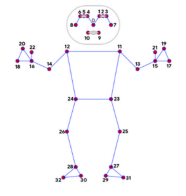
\includegraphics[width=\linewidth]{blazepose.png}
      \caption[BlazePose keypoints]{\label{fig:blazepose}BlazePose keypoints \autocite{RoggioEtAl2024}}
  \end{minipage}
  \hfill % Voegt wat ruimte toe tussen de afbeeldingen
  \begin{minipage}{0.45\textwidth}
      \centering
      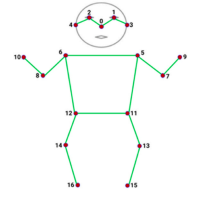
\includegraphics[width=\linewidth]{movenet.png}
      \caption[MoveNet keypoints]{\label{fig:movenet}MoveNet keypoints \autocite{RoggioEtAl2024}}
  \end{minipage}
\end{figure}  

\subsection{Conclusie}
MoveNet Lightning komt als beste keuze naar voren vanwege zijn uitzonderlijke snelheid (>50 FPS) en zijn optimale balans tussen prestaties en nauwkeurigheid. 
Zeker op mobiele apparaten, waar verwerkingscapaciteit en energieverbruik beperkt zijn, maakt deze efficiëntie een belangrijk verschil. 
Vergeleken met MoveNet Thunder, dat iets nauwkeuriger is, maar aanzienlijk trager, blijkt Lightning geschikter voor een realtime analyse-applicatie die feedback moet geven tijdens of vlak na de oefening.

\medskip

Deze configuratie maakt het mogelijk om technische fouten in krachttrainingsoefeningen objectief en onmiddellijk te detecteren, waardoor gebruikers hun uitvoering kunnen verbeteren en blessurerisico’s verlagen.